\documentclass[10pt]{standalone}
\usepackage{pgfplots}
\pgfplotsset{compat=1.15}
\usepackage{mathrsfs}
\usepackage{mlmodern}
\usetikzlibrary{arrows}
\pagestyle{empty}
\begin{document}%
\definecolor{ccqqqq}{rgb}{0.8,0.,0.}%
\definecolor{zzttqq}{rgb}{0.6,0.2,0.}%
\definecolor{wwwwww}{rgb}{0.4,0.4,0.4}%
\definecolor{cxvqqq}{rgb}{0.7803921568627451,0.3137254901960784,0.}%
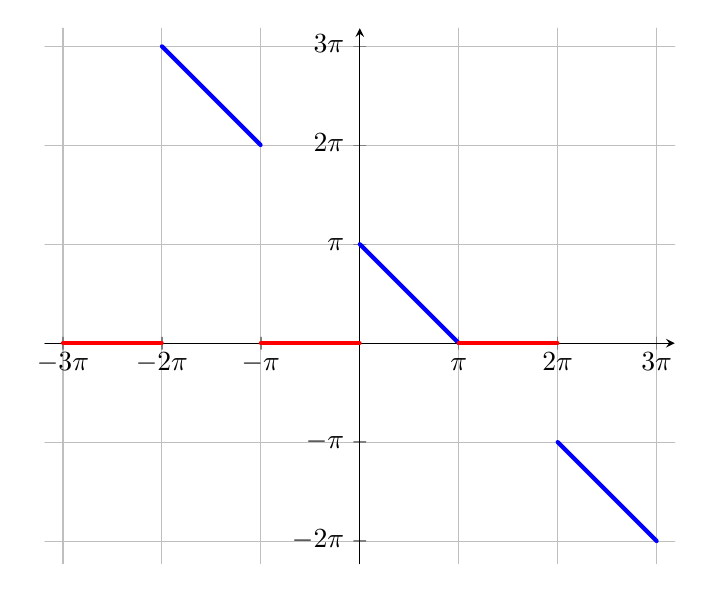
\begin{tikzpicture}[line cap=round,line join=round,>=triangle 45]
    \begin{axis}[
            x=.4cm,y=.4cm,
            axis lines=middle,
            ymajorgrids=true,
            xmajorgrids=true,
            xmin=-10.0,
            xmax=10.0,
            ymin=-7,
            ymax=10.0,
            xtick={-3*pi,-2*pi,...,3*pi},
            ytick={-2*pi,-1*pi,...,3*pi},
            xticklabels={$-3\pi$,$-2\pi$,$-\pi$,$0$,$\pi$,$2\pi$,$3\pi$},
            yticklabels={$-2\pi$,$-\pi$,$0$,$\pi$,$2\pi$,$3\pi$},
            ticklabel style={
                    text depth=0pt,
                    text height=1ex,
                },
            tick style={line width=.5pt}
        ]
        \clip(-10.,-10.) rectangle (10.,10.);
        \draw[line width=1.5pt,color=red] (-3.1415926000000023,0.0) -- (-0.007853988154731572,0.0);
        \draw[line width=1.5pt,color=blue] (0.0,3.1415926535897953) -- (3.1337360250000166,0.007856628589776538);
        \draw[line width=1.5pt,color=red] (3.1415928000000015,0.0) -- (6.275328262071768,0.0);
        \draw[line width=1.5pt,color=blue] (6.283185399999991,-3.141592746410198) -- (9.424774622060234,-6.283181968470441);
        \draw[line width=1.5pt,color=blue] (-6.283185200000037,9.42477785358983) -- (-3.1494467524739185,6.291039406063712);
        \draw[line width=1.5pt,color=red] (-9.424777799999983,0.0) -- (-6.291039351993112,0.0);
    \end{axis}
\end{tikzpicture}%
\end{document}